\section{Specification}
\label{sec:specification}
\subsection{Overview}
In the following I will describe the used architecture. 

Existing extractors as presented in Section~\ref{relatedWork} mostly suffer from their \textit{inflexible} nature resulting from their narrow use cases at development time. 
Very often approaches were only implemented to accomplish a short term goal (e.g. prove a scientific claim) and only the needed data was extracted in an \emph{ad-hoc} manner. 
Such evolutionary development generally makes it difficult to generalize the implementation to heterogeneous schemas of different WLE.
Most importantly, however, they ignore the community nature of a \wik. 
Fast changes of the data require ongoing maintenance, ideally by the wiki editors from the community itself or at least in tight collaboration with them.
These circumstances pose serious requirements to software design choices and should not be neglected. 
All existing tools are rather monolithic, hard-coded black boxes. 
Implementing a new WLE or making a major change in the WLE's ELE guidelines will require a programmer to refactor most of its application logic. 
Even small changes like new properties or naming conventions will require software engineers to align settings. 
The amount of maintenance work necessary for the extraction correlates with change frequency in the source. 
Following this argumentation, a community-built resource can only be efficiently extracted by a community-configured extractor. 
This argument is supported by the successful crowd-sourcing of DBpedia's internationalization~\cite{Kontokostas2012}  and the non-existence of \textit{open} alternatives with equal extensiveness.\\
Given these findings, we can now conclude four high-level design goals:
\begin{compactitem}
\item declarative description of the page schema;
\item declarative information/token extraction, using a terse syntax, maintainable by non-programmers;
\item configurable mapping from language-specific tokens to a global vocabulary;
\item fault tolerance (uninterpretable data is skipped).
\end{compactitem}

The extractor is built on top of the the DBpedia framework, and thus it is required to conform to a simple interface:

\begin{figure}[tb]
\centering
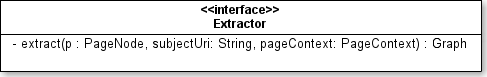
\includegraphics[width=0.6\textwidth]{./images/interface.png}
\caption{The extractor interface.}
\label{fig:interface}
\end{figure}

Extractors are registered with the framework via a configuration file, and instantiated with a requested context. The context can be the DBpedia ontology or the selected language etc. Extractors are then subsequently invoked for every page of the MediaWiki XML dump. They are given the page in parsed form of an AST, subjectURI the URI of the resource this page should be referring to (\texttt{http://dbpedia.org/resource/\$PAGENAME}) and pageContext --- a helper for URI generation. The interface defines the extractor to return a Graph in turn, which is basically a set of triples (or quads in this case). Internally the extractor will inspect the AST and generate triples, when he finds information he interprets as relevant. This straightforward interface makes the DBpedia framework so modular. Input and output handling (parsing and serialization) is left to the framework, and the resulting RDF data can be directly inserting into an triple store.

We solve the above requirements with an additional extractor, which internally follows a rather sophisticated workflow, shown in Figure~\ref{fig:architecture}.

\begin{figure}[htb]
\centering
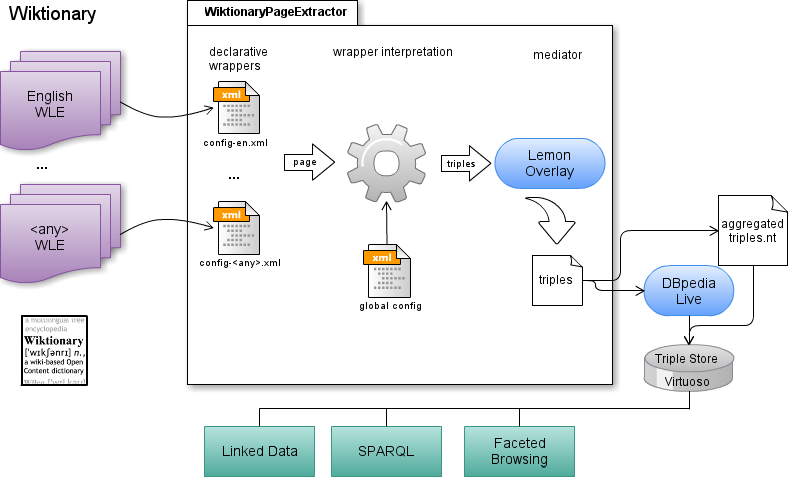
\includegraphics[width=0.9\textwidth]{./images/architecture.png}
\caption{Architecture for extracting semantics from Wiktionary leveraging the DBpedia framework.}
\label{fig:architecture}
\end{figure}
The \wik extractor is invoked by the DBpedia framework to handle a page.
It uses a language-specific configuration file, that has to be tailored to match the WLE's ELE guidelines to interpret the page, to extract the desired information. 
At first, the resulting triples still adhere to a language-specific schema, that directly reflects the configured layout of the WLE. 
A generic lossless transformation and annotation using the \lemon vocabulary is then applied to enforce a global schema and reduce semantic heterogeneity. 
Afterwards the triples are returned to the DBpedia frameworks, which takes care of the serialization and (optionally) the synchronization with a triple store via DBpedia Live\footnote{\url{http://live.dbpedia.org/live}} \cite{dbpedia_live_2012}.
The process of interpreting the declarative wrapper is explained in more detailed in Figure~\ref{fig:extractor}.

\begin{figure}[tb]
\centering
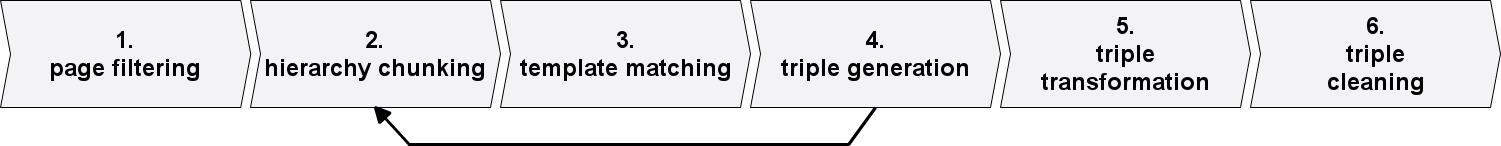
\includegraphics[width=0.9\textwidth]{./images/extractor.png}
\caption{Overview of the extractor workflow.}
\label{fig:extractor}
\end{figure}

The actual algorithm is quite complex and will be explained in more detail in the next section. What is important is, that separation in three phases: 
\begin{itemize}
\item preprocessing to skip pages that do not represent a lexical word
\item the actual extraction with the three steps of analyzing the page structure, matching templates and generating triple from the result
\item postprocessing to normalize schemata and polishing the output
\end{itemize}

The extractor itself is split into two components: a generic template matcher, that takes a (possibly partially consumed) wiki page and a template. It then tries to \textit{bind} the variable parts of the template to actual content from the page. When it a template is successfully matched, the matched part of the page is consumed --- removed from the page. This component is called the \texttt{VarBinder}. The VarBinder is a stateless tool that has no knowledge of the overall page layout 
\vfill
\newpage
